% Options for packages loaded elsewhere
\PassOptionsToPackage{unicode}{hyperref}
\PassOptionsToPackage{hyphens}{url}
%
\documentclass[
]{article}
\title{R Notebook}
\author{}
\date{\vspace{-2.5em}}

\usepackage{amsmath,amssymb}
\usepackage{lmodern}
\usepackage{iftex}
\ifPDFTeX
  \usepackage[T1]{fontenc}
  \usepackage[utf8]{inputenc}
  \usepackage{textcomp} % provide euro and other symbols
\else % if luatex or xetex
  \usepackage{unicode-math}
  \defaultfontfeatures{Scale=MatchLowercase}
  \defaultfontfeatures[\rmfamily]{Ligatures=TeX,Scale=1}
\fi
% Use upquote if available, for straight quotes in verbatim environments
\IfFileExists{upquote.sty}{\usepackage{upquote}}{}
\IfFileExists{microtype.sty}{% use microtype if available
  \usepackage[]{microtype}
  \UseMicrotypeSet[protrusion]{basicmath} % disable protrusion for tt fonts
}{}
\makeatletter
\@ifundefined{KOMAClassName}{% if non-KOMA class
  \IfFileExists{parskip.sty}{%
    \usepackage{parskip}
  }{% else
    \setlength{\parindent}{0pt}
    \setlength{\parskip}{6pt plus 2pt minus 1pt}}
}{% if KOMA class
  \KOMAoptions{parskip=half}}
\makeatother
\usepackage{xcolor}
\IfFileExists{xurl.sty}{\usepackage{xurl}}{} % add URL line breaks if available
\IfFileExists{bookmark.sty}{\usepackage{bookmark}}{\usepackage{hyperref}}
\hypersetup{
  pdftitle={R Notebook},
  hidelinks,
  pdfcreator={LaTeX via pandoc}}
\urlstyle{same} % disable monospaced font for URLs
\usepackage[margin=1in]{geometry}
\usepackage{color}
\usepackage{fancyvrb}
\newcommand{\VerbBar}{|}
\newcommand{\VERB}{\Verb[commandchars=\\\{\}]}
\DefineVerbatimEnvironment{Highlighting}{Verbatim}{commandchars=\\\{\}}
% Add ',fontsize=\small' for more characters per line
\usepackage{framed}
\definecolor{shadecolor}{RGB}{248,248,248}
\newenvironment{Shaded}{\begin{snugshade}}{\end{snugshade}}
\newcommand{\AlertTok}[1]{\textcolor[rgb]{0.94,0.16,0.16}{#1}}
\newcommand{\AnnotationTok}[1]{\textcolor[rgb]{0.56,0.35,0.01}{\textbf{\textit{#1}}}}
\newcommand{\AttributeTok}[1]{\textcolor[rgb]{0.77,0.63,0.00}{#1}}
\newcommand{\BaseNTok}[1]{\textcolor[rgb]{0.00,0.00,0.81}{#1}}
\newcommand{\BuiltInTok}[1]{#1}
\newcommand{\CharTok}[1]{\textcolor[rgb]{0.31,0.60,0.02}{#1}}
\newcommand{\CommentTok}[1]{\textcolor[rgb]{0.56,0.35,0.01}{\textit{#1}}}
\newcommand{\CommentVarTok}[1]{\textcolor[rgb]{0.56,0.35,0.01}{\textbf{\textit{#1}}}}
\newcommand{\ConstantTok}[1]{\textcolor[rgb]{0.00,0.00,0.00}{#1}}
\newcommand{\ControlFlowTok}[1]{\textcolor[rgb]{0.13,0.29,0.53}{\textbf{#1}}}
\newcommand{\DataTypeTok}[1]{\textcolor[rgb]{0.13,0.29,0.53}{#1}}
\newcommand{\DecValTok}[1]{\textcolor[rgb]{0.00,0.00,0.81}{#1}}
\newcommand{\DocumentationTok}[1]{\textcolor[rgb]{0.56,0.35,0.01}{\textbf{\textit{#1}}}}
\newcommand{\ErrorTok}[1]{\textcolor[rgb]{0.64,0.00,0.00}{\textbf{#1}}}
\newcommand{\ExtensionTok}[1]{#1}
\newcommand{\FloatTok}[1]{\textcolor[rgb]{0.00,0.00,0.81}{#1}}
\newcommand{\FunctionTok}[1]{\textcolor[rgb]{0.00,0.00,0.00}{#1}}
\newcommand{\ImportTok}[1]{#1}
\newcommand{\InformationTok}[1]{\textcolor[rgb]{0.56,0.35,0.01}{\textbf{\textit{#1}}}}
\newcommand{\KeywordTok}[1]{\textcolor[rgb]{0.13,0.29,0.53}{\textbf{#1}}}
\newcommand{\NormalTok}[1]{#1}
\newcommand{\OperatorTok}[1]{\textcolor[rgb]{0.81,0.36,0.00}{\textbf{#1}}}
\newcommand{\OtherTok}[1]{\textcolor[rgb]{0.56,0.35,0.01}{#1}}
\newcommand{\PreprocessorTok}[1]{\textcolor[rgb]{0.56,0.35,0.01}{\textit{#1}}}
\newcommand{\RegionMarkerTok}[1]{#1}
\newcommand{\SpecialCharTok}[1]{\textcolor[rgb]{0.00,0.00,0.00}{#1}}
\newcommand{\SpecialStringTok}[1]{\textcolor[rgb]{0.31,0.60,0.02}{#1}}
\newcommand{\StringTok}[1]{\textcolor[rgb]{0.31,0.60,0.02}{#1}}
\newcommand{\VariableTok}[1]{\textcolor[rgb]{0.00,0.00,0.00}{#1}}
\newcommand{\VerbatimStringTok}[1]{\textcolor[rgb]{0.31,0.60,0.02}{#1}}
\newcommand{\WarningTok}[1]{\textcolor[rgb]{0.56,0.35,0.01}{\textbf{\textit{#1}}}}
\usepackage{graphicx}
\makeatletter
\def\maxwidth{\ifdim\Gin@nat@width>\linewidth\linewidth\else\Gin@nat@width\fi}
\def\maxheight{\ifdim\Gin@nat@height>\textheight\textheight\else\Gin@nat@height\fi}
\makeatother
% Scale images if necessary, so that they will not overflow the page
% margins by default, and it is still possible to overwrite the defaults
% using explicit options in \includegraphics[width, height, ...]{}
\setkeys{Gin}{width=\maxwidth,height=\maxheight,keepaspectratio}
% Set default figure placement to htbp
\makeatletter
\def\fps@figure{htbp}
\makeatother
\setlength{\emergencystretch}{3em} % prevent overfull lines
\providecommand{\tightlist}{%
  \setlength{\itemsep}{0pt}\setlength{\parskip}{0pt}}
\setcounter{secnumdepth}{-\maxdimen} % remove section numbering
\ifLuaTeX
  \usepackage{selnolig}  % disable illegal ligatures
\fi

\begin{document}
\maketitle

This is an \href{http://rmarkdown.rstudio.com}{R Markdown} Notebook.
When you execute code within the notebook, the results appear beneath
the code.

Try executing this chunk by clicking the \emph{Run} button within the
chunk or by placing your cursor inside it and pressing
\emph{Ctrl+Shift+Enter}.

\#\#Importe les données

\begin{Shaded}
\begin{Highlighting}[]
\NormalTok{df\_employee\_survey\_data }\OtherTok{\textless{}{-}} \FunctionTok{read.csv}\NormalTok{(}\StringTok{\textquotesingle{}C://Users//louis//Documents//COURS EMSE//Année 5 {-} Ingé 3//ESME//R//Projet//archive//employee\_survey\_data.csv\textquotesingle{}}\NormalTok{)}
\NormalTok{df\_general\_data}\OtherTok{\textless{}{-}} \FunctionTok{read.csv}\NormalTok{(}\StringTok{\textquotesingle{}C://Users//louis//Documents//COURS EMSE//Année 5 {-} Ingé 3//ESME//R//Projet//archive//general\_data.csv\textquotesingle{}}\NormalTok{)}
\NormalTok{df\_in\_time}\OtherTok{\textless{}{-}} \FunctionTok{read.csv}\NormalTok{(}\StringTok{\textquotesingle{}C://Users//louis//Documents//COURS EMSE//Année 5 {-} Ingé 3//ESME//R//Projet//archive//in\_time.csv\textquotesingle{}}\NormalTok{)}
\NormalTok{df\_manager\_survey\_data}\OtherTok{\textless{}{-}} \FunctionTok{read.csv}\NormalTok{(}\StringTok{\textquotesingle{}C://Users//louis//Documents//COURS EMSE//Année 5 {-} Ingé 3//ESME//R//Projet//archive//manager\_survey\_data.csv\textquotesingle{}}\NormalTok{)}
\NormalTok{df\_out\_time}\OtherTok{\textless{}{-}} \FunctionTok{read.csv}\NormalTok{(}\StringTok{\textquotesingle{}C://Users//louis//Documents//COURS EMSE//Année 5 {-} Ingé 3//ESME//R//Projet//archive//out\_time.csv\textquotesingle{}}\NormalTok{)}
\end{Highlighting}
\end{Shaded}

\begin{Shaded}
\begin{Highlighting}[]
\FunctionTok{head}\NormalTok{(df\_employee\_survey\_data)}
\end{Highlighting}
\end{Shaded}

\begin{verbatim}
##   EmployeeID EnvironmentSatisfaction JobSatisfaction WorkLifeBalance
## 1          1                       3               4               2
## 2          2                       3               2               4
## 3          3                       2               2               1
## 4          4                       4               4               3
## 5          5                       4               1               3
## 6          6                       3               2               2
\end{verbatim}

\#Traitement des données

\#\#Vérifie s'il y a des valeurs manquantes

\#Premier dataframe : df\_employee\_survey\_data

\begin{Shaded}
\begin{Highlighting}[]
\FunctionTok{colSums}\NormalTok{(}\FunctionTok{is.na}\NormalTok{(df\_employee\_survey\_data))}
\end{Highlighting}
\end{Shaded}

\begin{verbatim}
##              EmployeeID EnvironmentSatisfaction         JobSatisfaction 
##                       0                      25                      20 
##         WorkLifeBalance 
##                      38
\end{verbatim}

\#Second dataframe : df\_general\_data Add a new chunk by clicking the
\emph{Insert Chunk} button on the toolbar or by pressing
\emph{Ctrl+Alt+I}.

\begin{Shaded}
\begin{Highlighting}[]
\FunctionTok{colSums}\NormalTok{(}\FunctionTok{is.na}\NormalTok{(df\_general\_data))}
\end{Highlighting}
\end{Shaded}

\begin{verbatim}
##                     Age               Attrition          BusinessTravel 
##                       0                       0                       0 
##              Department        DistanceFromHome               Education 
##                       0                       0                       0 
##          EducationField           EmployeeCount              EmployeeID 
##                       0                       0                       0 
##                  Gender                JobLevel                 JobRole 
##                       0                       0                       0 
##           MaritalStatus           MonthlyIncome      NumCompaniesWorked 
##                       0                       0                      19 
##                  Over18       PercentSalaryHike           StandardHours 
##                       0                       0                       0 
##        StockOptionLevel       TotalWorkingYears   TrainingTimesLastYear 
##                       0                       9                       0 
##          YearsAtCompany YearsSinceLastPromotion    YearsWithCurrManager 
##                       0                       0                       0
\end{verbatim}

\#Troisième : In\_time \& Out\_time Dataframe

\begin{Shaded}
\begin{Highlighting}[]
\CommentTok{\#A cause de l\textquotesingle{}immense quantité de données présente on ne peut pas juste afficher les colonnes avec le nombre de Na. Cela serait ilisible. }

\FunctionTok{any}\NormalTok{(}\FunctionTok{is.na}\NormalTok{(df\_in\_time))}
\end{Highlighting}
\end{Shaded}

\begin{verbatim}
## [1] TRUE
\end{verbatim}

\begin{Shaded}
\begin{Highlighting}[]
\FunctionTok{any}\NormalTok{(}\FunctionTok{is.na}\NormalTok{(df\_out\_time))}
\end{Highlighting}
\end{Shaded}

\begin{verbatim}
## [1] TRUE
\end{verbatim}

\#Quatrième : df\_manager\_survey\_data When you save the notebook, an
HTML file containing the code and output will be saved alongside it
(click the \emph{Preview} button or press \emph{Ctrl+Shift+K} to preview
the HTML file).

\begin{Shaded}
\begin{Highlighting}[]
\FunctionTok{colSums}\NormalTok{(}\FunctionTok{is.na}\NormalTok{(df\_manager\_survey\_data))}
\end{Highlighting}
\end{Shaded}

\begin{verbatim}
##        EmployeeID    JobInvolvement PerformanceRating 
##                 0                 0                 0
\end{verbatim}

\#Remplacement des données Manquantes par la Moyenne \#\#\#Afin de ne
pas fausser notre jeux de données en supprimant simplement les lignes
incomplètes nous allons remplacer les Na par la moyenne.

\begin{Shaded}
\begin{Highlighting}[]
\CommentTok{\#duplique le dataframe afin d\textquotesingle{}effectuer nos essaie }
\NormalTok{df\_test }\OtherTok{\textless{}{-}}\NormalTok{ df\_general\_data}
\NormalTok{df\_test}\SpecialCharTok{$}\NormalTok{NumCompaniesWorked[}\FunctionTok{is.na}\NormalTok{(df\_test}\SpecialCharTok{$}\NormalTok{NumCompaniesWorked)] }\OtherTok{\textless{}{-}} \FunctionTok{mean}\NormalTok{(df\_test}\SpecialCharTok{$}\NormalTok{NumCompaniesWorked, }\AttributeTok{na.rm =} \ConstantTok{TRUE}\NormalTok{)}
\CommentTok{\# na.rm =TRUE : retire les Na du calcul de la moyenne }
\FunctionTok{colSums}\NormalTok{(}\FunctionTok{is.na}\NormalTok{(df\_test))}
\end{Highlighting}
\end{Shaded}

\begin{verbatim}
##                     Age               Attrition          BusinessTravel 
##                       0                       0                       0 
##              Department        DistanceFromHome               Education 
##                       0                       0                       0 
##          EducationField           EmployeeCount              EmployeeID 
##                       0                       0                       0 
##                  Gender                JobLevel                 JobRole 
##                       0                       0                       0 
##           MaritalStatus           MonthlyIncome      NumCompaniesWorked 
##                       0                       0                       0 
##                  Over18       PercentSalaryHike           StandardHours 
##                       0                       0                       0 
##        StockOptionLevel       TotalWorkingYears   TrainingTimesLastYear 
##                       0                       9                       0 
##          YearsAtCompany YearsSinceLastPromotion    YearsWithCurrManager 
##                       0                       0                       0
\end{verbatim}

\begin{Shaded}
\begin{Highlighting}[]
\CommentTok{\#Colonne NumCompaniesWorked}
\NormalTok{df\_general\_data}\SpecialCharTok{$}\NormalTok{NumCompaniesWorked[}\FunctionTok{is.na}\NormalTok{(df\_general\_data}\SpecialCharTok{$}\NormalTok{NumCompaniesWorked)] }\OtherTok{\textless{}{-}} \FunctionTok{mean}\NormalTok{(df\_test}\SpecialCharTok{$}\NormalTok{NumCompaniesWorked, }\AttributeTok{na.rm =} \ConstantTok{TRUE}\NormalTok{)}

\CommentTok{\#Colonne TotalWorkingYears}

\NormalTok{df\_general\_data}\SpecialCharTok{$}\NormalTok{TotalWorkingYears[}\FunctionTok{is.na}\NormalTok{(df\_general\_data}\SpecialCharTok{$}\NormalTok{TotalWorkingYears)] }\OtherTok{\textless{}{-}} \FunctionTok{mean}\NormalTok{(df\_test}\SpecialCharTok{$}\NormalTok{TotalWorkingYears, }\AttributeTok{na.rm =} \ConstantTok{TRUE}\NormalTok{)}

\FunctionTok{any}\NormalTok{(}\FunctionTok{is.na}\NormalTok{(df\_general\_data))}
\end{Highlighting}
\end{Shaded}

\begin{verbatim}
## [1] FALSE
\end{verbatim}

\#Exploiration des données générales

\#\#Roulement du personnel

\begin{Shaded}
\begin{Highlighting}[]
\CommentTok{\#data \textless{}{-} table(df\_general\_data[\textquotesingle{}Attrition\textquotesingle{}])   affiche les données en somme }
\NormalTok{data }\OtherTok{\textless{}{-}} \FunctionTok{prop.table}\NormalTok{(}\FunctionTok{table}\NormalTok{(df\_general\_data[}\StringTok{\textquotesingle{}Attrition\textquotesingle{}}\NormalTok{]))}\SpecialCharTok{*}\DecValTok{100}   \CommentTok{\#affiche porucentage }


\FunctionTok{barplot}\NormalTok{ (data , }\AttributeTok{space =}\FloatTok{1.0}\NormalTok{,}
         \AttributeTok{main=}\StringTok{"Attrition"}\NormalTok{,  }\CommentTok{\#Nom graph}
         \AttributeTok{ylim=}\FunctionTok{c}\NormalTok{(}\DecValTok{0}\NormalTok{,}\DecValTok{100}\NormalTok{))     }\CommentTok{\#échelle des ordonnées}
\end{Highlighting}
\end{Shaded}

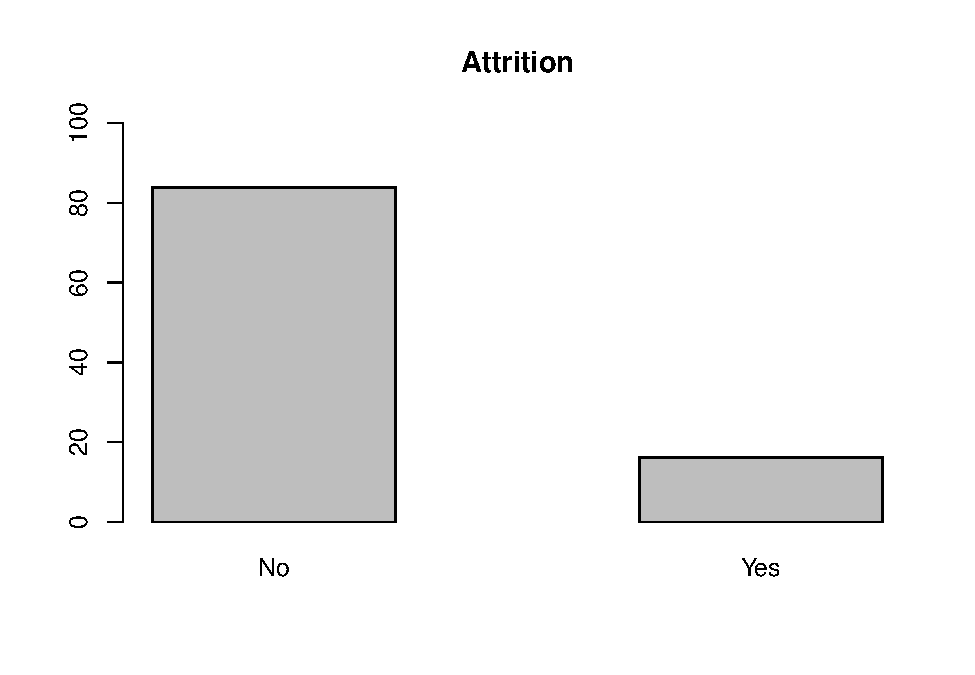
\includegraphics{Projet_files/figure-latex/unnamed-chunk-9-1.pdf}
\#Analyse Salaire

\#Répartitions des salaires

\begin{Shaded}
\begin{Highlighting}[]
\FunctionTok{boxplot}\NormalTok{(df\_general\_data}\SpecialCharTok{$}\NormalTok{MonthlyIncome,}
        \AttributeTok{main =} \StringTok{\textquotesingle{}Box Plot: Salaire\textquotesingle{}}\NormalTok{,}
        \AttributeTok{xlab=}\StringTok{"salaire mensuel ($)"}\NormalTok{)}
\end{Highlighting}
\end{Shaded}

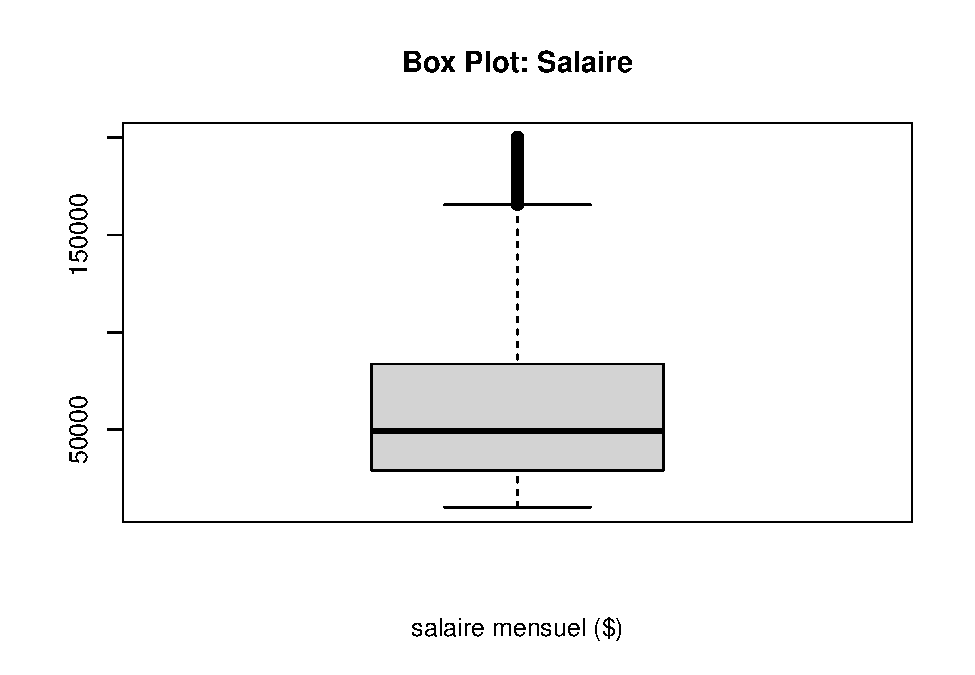
\includegraphics{Projet_files/figure-latex/unnamed-chunk-10-1.pdf}

\begin{Shaded}
\begin{Highlighting}[]
\FunctionTok{boxplot}\NormalTok{(df\_general\_data}\SpecialCharTok{$}\NormalTok{MonthlyIncome }\SpecialCharTok{\textasciitilde{}}\NormalTok{ df\_general\_data}\SpecialCharTok{$}\NormalTok{Department, }
        \AttributeTok{main=}\StringTok{\textquotesingle{}salire en fonction du déârtement\textquotesingle{}}\NormalTok{,}
        \AttributeTok{ylab=}\StringTok{"salaire mensuel ($)"}\NormalTok{,}
        \AttributeTok{xlab=}\StringTok{"Département"}\NormalTok{)}
\end{Highlighting}
\end{Shaded}

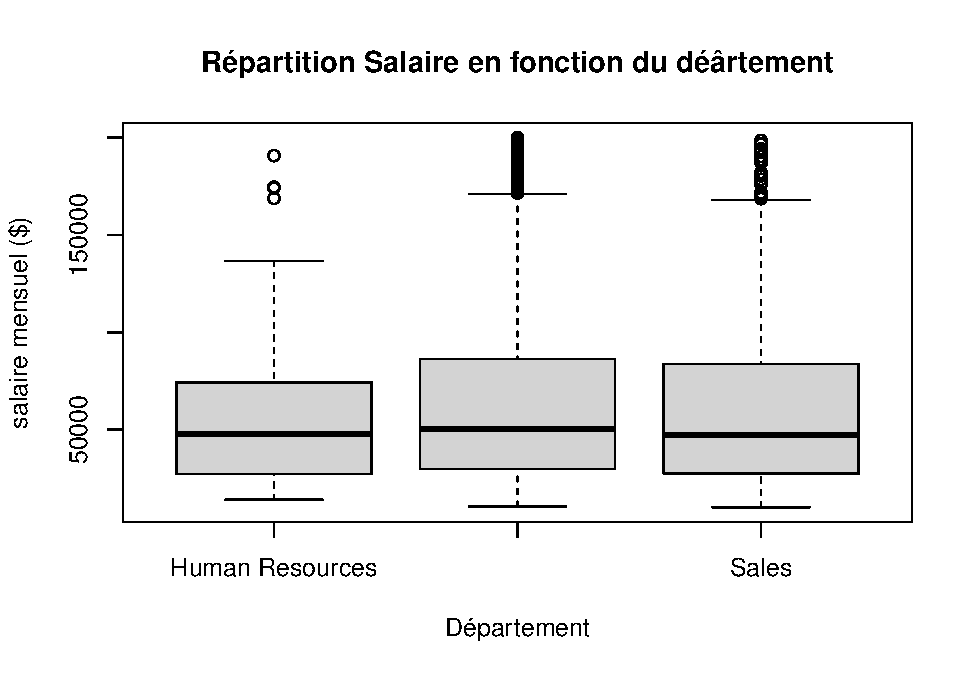
\includegraphics{Projet_files/figure-latex/unnamed-chunk-10-2.pdf}

\begin{Shaded}
\begin{Highlighting}[]
\FunctionTok{boxplot}\NormalTok{(df\_general\_data}\SpecialCharTok{$}\NormalTok{MonthlyIncome }\SpecialCharTok{\textasciitilde{}}\NormalTok{ df\_general\_data}\SpecialCharTok{$}\NormalTok{JobRole,}
        \AttributeTok{las=}\DecValTok{2}\NormalTok{,   }\CommentTok{\#légende à la verticale}
        \AttributeTok{main=}\StringTok{\textquotesingle{}Salaire en fonction du poste\textquotesingle{}}\NormalTok{,}
        \AttributeTok{ylab=}\StringTok{"salaire mensuel ($)"}\NormalTok{,}
        \AttributeTok{xlab=}\StringTok{"Postes"}\NormalTok{)}
\end{Highlighting}
\end{Shaded}

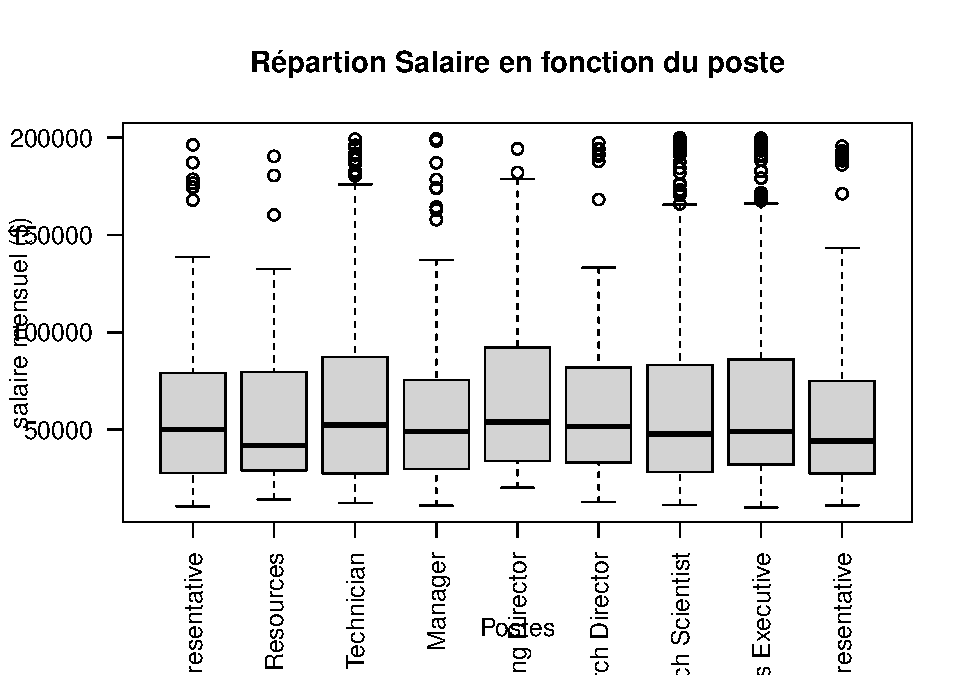
\includegraphics{Projet_files/figure-latex/unnamed-chunk-10-3.pdf}

\#\#Revenue en fonction du post

The preview shows you a rendered HTML copy of the contents of the
editor. Consequently, unlike \emph{Knit}, \emph{Preview} does not run
any R code chunks. Instead, the output of the chunk when it was last run
in the editor is displayed.

\end{document}
